\chapter{Results and Discussion}
\label{ch:results}

This chapter gives our results. Sections~\ref{sec:setup}--\ref{sec:qual} contain the \textbf{measured results} of the two Kaggle runs, copied directly from the outputs of the notebooks we submit: configuration~A (\texttt{mini-6\_working}) and configuration~B (\texttt{mini-7-fixed}). Section~\ref{sec:local} adds the results of the smaller \emph{local} run made with the packaged system on a laptop. Section~\ref{sec:reported} then shows, separately, the \textbf{numbers given in our earlier IEEE-style paper draft}. Those numbers are higher than anything our code produced and we could not reproduce them, so every table and figure taken from the draft carries the label ``Reported in paper draft'' and the mark~\reportedtag. Section~\ref{sec:discussion} discusses all of these results together.

\section{Experimental Setup}
\label{sec:setup}

\subsection{Configurations}
We ran the whole pipeline twice on Kaggle's two T4 GPUs. Both runs use the code of Chapter~\ref{ch:impl}; they differ only in the data mix and the settings (Tables~\ref{tab:rm-hparams} and~\ref{tab:dpo-hparams}):
\begin{itemize}
  \item \textbf{Configuration A (balanced):} 2,000 pairs from each source. Reward model with LoRA rank 32, two epochs, learning rate $2\times10^{-5}$. DPO on 1,500 pairs with rank-16 LoRA on the attention layers only, learning rate $5\times10^{-5}$, $\beta$=0.1, two epochs.
  \item \textbf{Configuration B (more HH-RLHF):} 6,000 HH-RLHF and 2,000 LMSYS pairs. Reward model with LoRA rank 64, three epochs, learning rate $1\times10^{-5}$. DPO on 3,000 pairs (two HH-RLHF for every LMSYS pair) with rank-32 LoRA on attention and feed-forward layers, learning rate $1\times10^{-5}$, $\beta$=0.15, keeping the checkpoint with the best validation loss.
\end{itemize}

\subsection{Evaluation protocol}
\begin{enumerate}
  \item \textbf{RM evaluation:} pairwise accuracy and mean reward gap on the full held-out test split (250 pairs in A, 500 in B), overall and per source.
  \item \textbf{Demo reel:} five fixed prompts (two factual, one study-skills, two socio-emotional), one sample per model, scored by the RM.
  \item \textbf{Held-out evaluation:} 25 HH-RLHF and 25 LMSYS prompts sampled from the test split with seed 42; one sample per model per prompt; win rate and mean $\Delta$ overall and per source.
  \item \textbf{Interactive session (config.\ A):} seven prompts typed live during a demonstration.
\end{enumerate}

\subsection{Statistical resolution}
Our test sets are small, so it helps to know how much a percentage can move by chance alone. For $n$ yes/no outcomes near 50\%, a 95\% interval is roughly $\pm1.96\sqrt{0.25/n}$. That is about $\pm$13.9 points for 50 prompts and $\pm$19.6 points for 25. A difference in win rate smaller than this should not be read as a real effect. For the reward-model test sets the margins are about $\pm$6.1 points ($n$=250), $\pm$4.3 ($n$=500), $\pm$5.0 ($n$=375) and $\pm$8.6 ($n$=125).

\section{Dataset Analysis}
\label{sec:res-data}

Figures~\ref{fig:m6-dataset} and~\ref{fig:m7-dataset} describe the training data of the two configurations. Prompt lengths look similar for both sources, but LMSYS chosen answers are clearly longer than HH-RLHF ones, and their long tail is cut at 1,500 characters. Because the two sources differ this much in length, a reward model that learned ``longer is better'' from LMSYS might carry that rule over to HH-RLHF. Checking each source separately is how we would notice.

\begin{figure}[H]
\centering
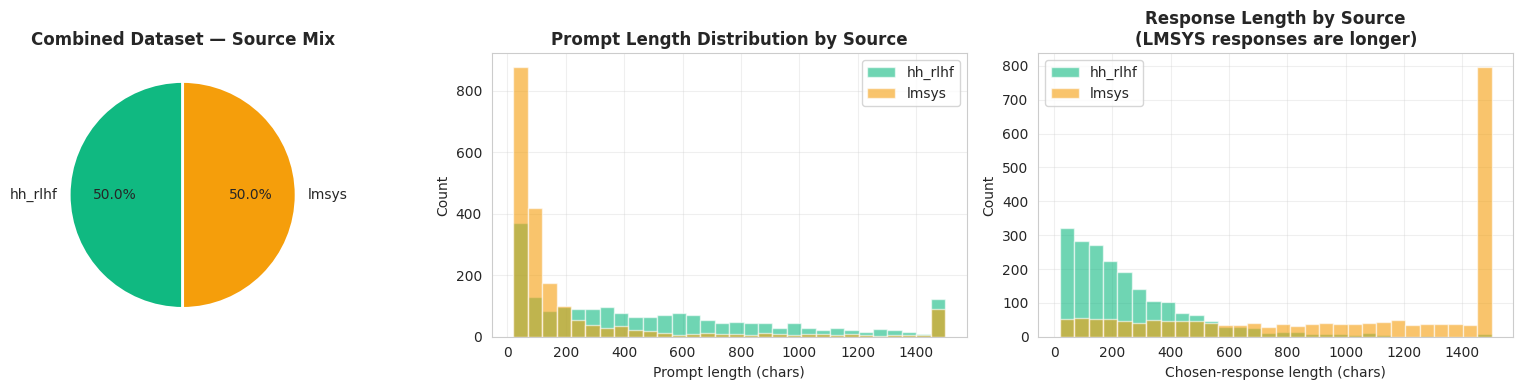
\includegraphics[width=\textwidth]{figures/m6_14_1.png}
\caption[Dataset composition, configuration A]{Configuration A dataset composition: (a) 50/50 source mix, (b) prompt length and (c) chosen-response length by source (measured, \texttt{mini-6}).}
\label{fig:m6-dataset}
\end{figure}

\begin{figure}[H]
\centering
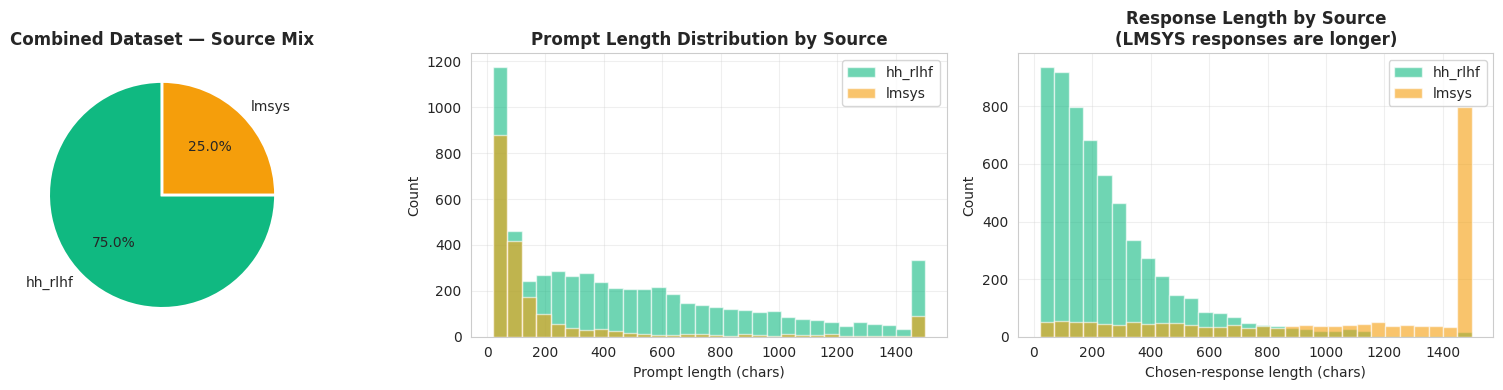
\includegraphics[width=\textwidth]{figures/m7_14_1.png}
\caption[Dataset composition, configuration B]{Configuration B dataset composition: 75/25 HH-RLHF/LMSYS mix (measured, \texttt{mini-7}).}
\label{fig:m7-dataset}
\end{figure}

\section{Reward Model Results}
\label{sec:res-rm}

\subsection{Training dynamics}
Figures~\ref{fig:m6-rmloss} and~\ref{fig:m7-rmloss} plot the reward model's training and validation loss. Both start at $\log 2\approx0.693$, which is what a model that cannot tell the two answers apart scores. In configuration A the validation loss reaches about 0.667 after roughly 210 steps (two epochs with 32 pairs per step). Configuration B, with twice the data and three epochs, reaches about 0.653 after roughly 650 steps, but stops improving after step 400 while the training loss keeps jumping up and down. Neither curve diverges. The improvement is small, though: a loss of 0.653 means the model gives the correct answer an average probability of only about $e^{-0.653}\approx0.52$. It is right more often than wrong, but not by much.

\begin{figure}[H]
\centering
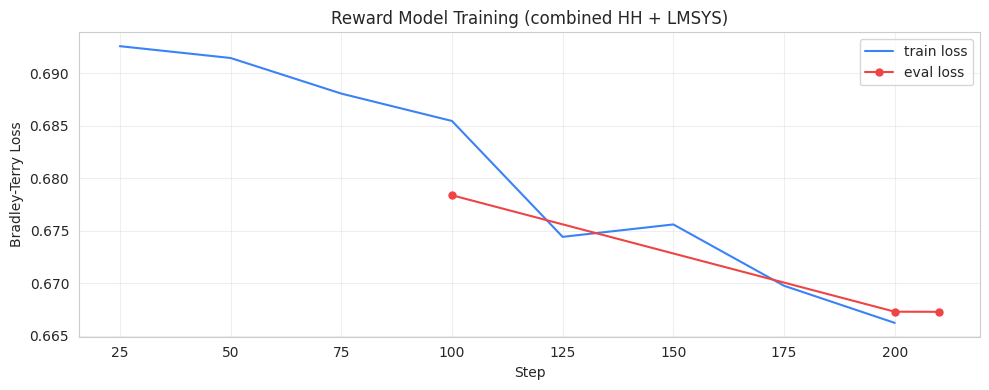
\includegraphics[width=0.85\textwidth]{figures/m6_25_3.png}
\caption[Reward-model loss, configuration A]{Reward-model training and validation loss, configuration A (measured).}
\label{fig:m6-rmloss}
\end{figure}

\begin{figure}[H]
\centering
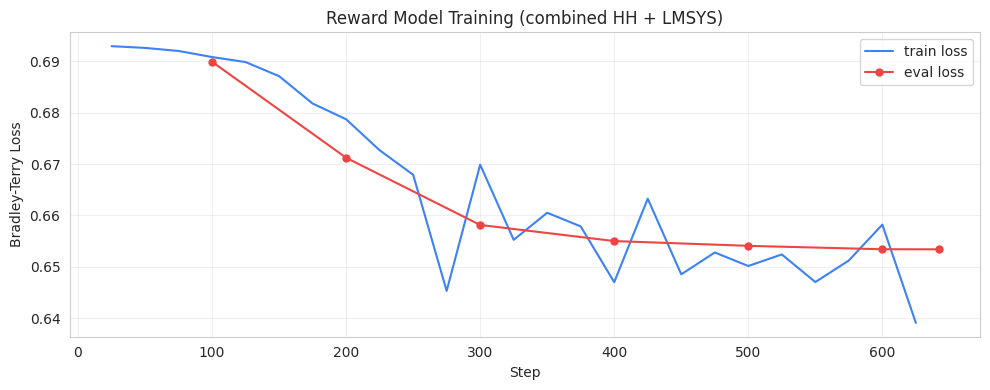
\includegraphics[width=0.85\textwidth]{figures/m7_25_3.png}
\caption[Reward-model loss, configuration B]{Reward-model training and validation loss, configuration B (measured).}
\label{fig:m7-rmloss}
\end{figure}

\subsection{Held-out test accuracy}
Table~\ref{tab:rm-results} gives the per-source test results of both configurations, as printed by the notebooks.

\begin{table}[!htbp]
\centering
\caption[Reward-model test results (A and B)]{Reward-model evaluation on the held-out test split (measured). The gap is the mean of chosen minus rejected reward.}
\label{tab:rm-results}
\small\setlength{\tabcolsep}{4.5pt}
\begin{tabular}{@{}llrrrrc@{}}
\toprule
\textbf{Config.} & \textbf{Split} & \textbf{$n$} & \textbf{Chosen $\bar r$} & \textbf{Rejected $\bar r$} & \textbf{Gap} & \textbf{Pairwise acc.}\\
\midrule
\multirow{3}{*}{A (2K+2K)} & Combined & 250 & $-0.4744$ & $-0.5432$ & $+0.0688$ & \textbf{59.2\%}\\
 & HH-RLHF & 125 & $-0.6847$ & $-0.7237$ & $+0.0390$ & 59.2\%\\
 & LMSYS & 125 & $-0.2642$ & $-0.3627$ & $+0.0985$ & 59.2\%\\
\midrule
\multirow{3}{*}{B (6K+2K)} & Combined & 500 & $-0.5502$ & $-0.6677$ & $+0.1175$ & \textbf{59.6\%}\\
 & HH-RLHF & 375 & $-0.6931$ & $-0.8124$ & $+0.1192$ & 57.9\%\\
 & LMSYS & 125 & $-0.1215$ & $-0.2337$ & $+0.1122$ & 64.8\%\\
\midrule
-- & Random baseline & -- & -- & -- & 0 & 50.0\%\\
\bottomrule
\end{tabular}
\end{table}

\paragraph{Better than guessing.} Both reward models beat the 50\% baseline by more than the margin of error; the 95\% intervals are about [53\%, 65\%] for A and [55\%, 64\%] for B. In every subset the average score of chosen answers is above that of rejected answers, which is the pass condition we set in the notebook.

\paragraph{Balance between sources.} In configuration A the reward model gets \emph{exactly} the same accuracy on both sources, 74 correct out of 125 each. In configuration B the gap is 6.9 points (57.9\% against 64.8\%). Both are inside our 10-point limit, so neither model has locked onto one source. The direction of B's gap surprised us: B saw three times more HH-RLHF pairs than LMSYS pairs, yet it does better on LMSYS. Our explanation is that an LMSYS pair often compares answers from two quite different chatbots, which is easier to judge, whereas the two answers in an HH-RLHF pair come from very similar Anthropic models and are often nearly the same.

\paragraph{More data did not help much.} Going from A to B, with three times the HH-RLHF data and one more epoch, made the model more confident (average gap 0.069 to 0.118) but hardly more accurate (59.2\% to 59.6\%). At this scale, a 184M-parameter encoder on a few thousand noisy pairs seems limited by its size and by the label noise rather than by the amount of data.

\subsection{Score distributions}
Figures~\ref{fig:m6-rmdist} and~\ref{fig:m7-rmdist} show how the scores and the per-pair gaps are spread. The chosen and rejected histograms overlap a lot, and the gap histograms sit only slightly to the right of zero, which fits a weak but real signal. In configuration A a large group of LMSYS scores bunches up near the top of the range (about $+0.1$), as if the classifier output saturates for some inputs.

\begin{figure}[H]
\centering
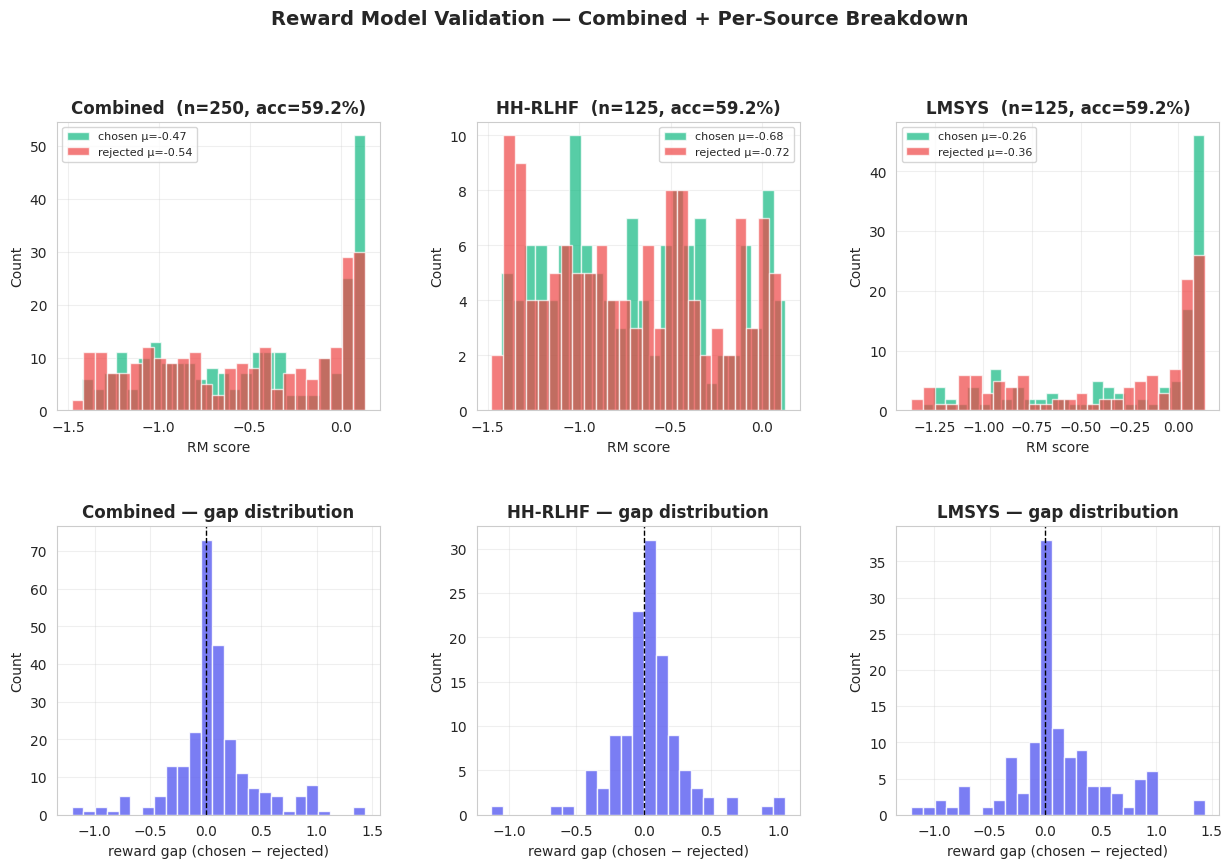
\includegraphics[width=\textwidth]{figures/m6_24_2.png}
\caption[Reward-model score distributions, configuration A]{Configuration A reward-model validation: score histograms (top) and gap distributions (bottom) for the combined, HH-RLHF and LMSYS test subsets (measured).}
\label{fig:m6-rmdist}
\end{figure}

\begin{figure}[H]
\centering
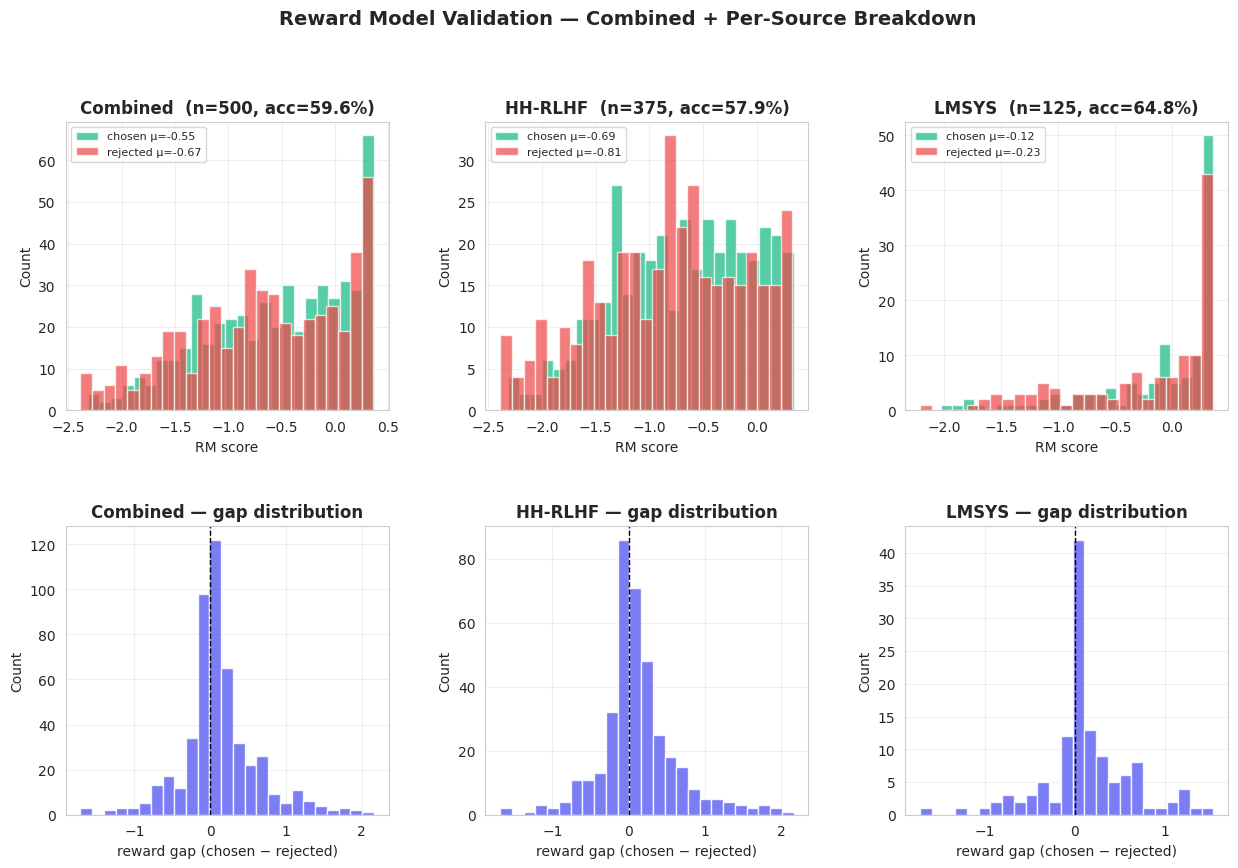
\includegraphics[width=\textwidth]{figures/m7_24_2.png}
\caption[Reward-model score distributions, configuration B]{Configuration B reward-model validation: score histograms and gap distributions per subset (measured).}
\label{fig:m7-rmdist}
\end{figure}

\section{DPO Training Results}
\label{sec:res-dpo-train}

Figures~\ref{fig:m6-dpocurves} and~\ref{fig:m7-dpocurves} show the DPO training diagnostics logged by TRL: loss, mean implicit rewards of chosen and rejected responses, and implicit-reward accuracy.

\begin{figure}[H]
\centering
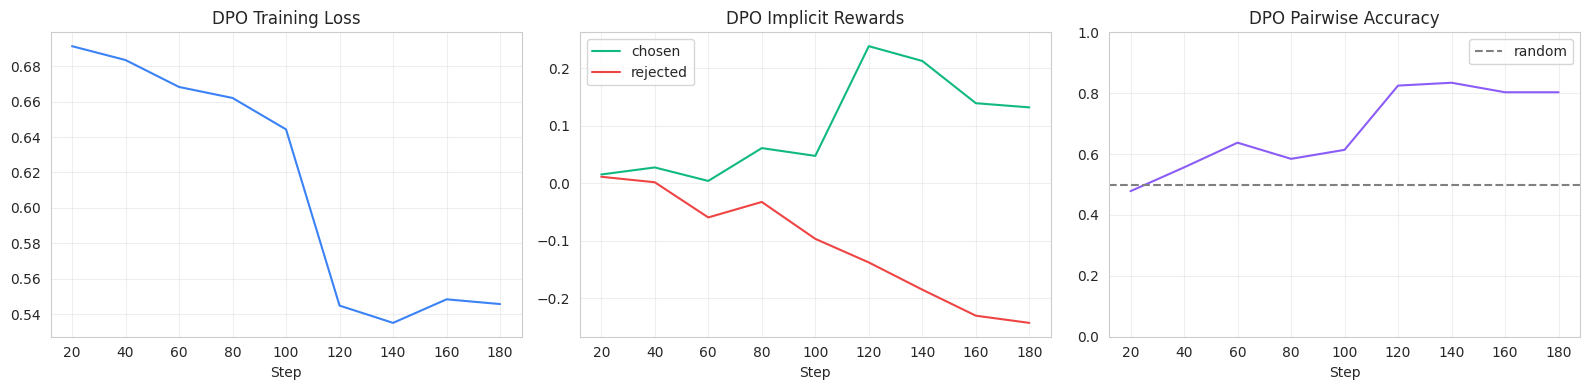
\includegraphics[width=\textwidth]{figures/m6_32_4.png}
\caption[DPO training curves, configuration A]{DPO training curves, configuration A: loss, implicit rewards and implicit-reward accuracy (measured).}
\label{fig:m6-dpocurves}
\end{figure}

\begin{figure}[H]
\centering
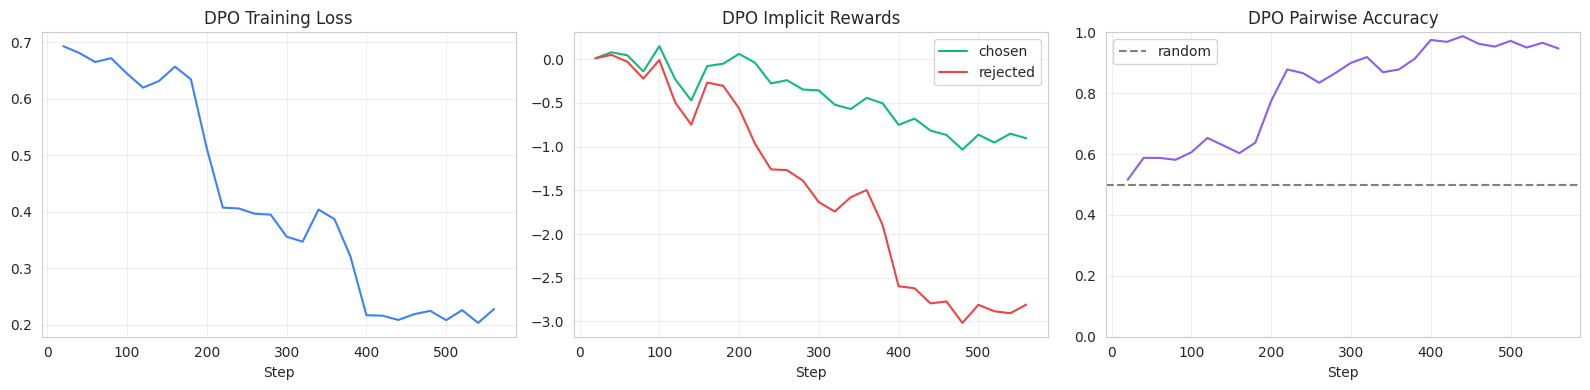
\includegraphics[width=\textwidth]{figures/m7_32_4.png}
\caption[DPO training curves, configuration B]{DPO training curves, configuration B (measured).}
\label{fig:m7-dpocurves}
\end{figure}

In configuration A the loss drops from 0.69 to about 0.54 in roughly 190 steps. The implicit reward of chosen answers climbs to about $+0.13$ and that of rejected answers falls to about $-0.24$, so the two move apart as intended, and the share of pairs ranked correctly rises from chance to about 80\%. Configuration B trains for about 560 steps and goes much further: the loss falls to about 0.2 and accuracy reaches about 95\% (Table~\ref{tab:dpo-log}). In B, however, \emph{both} implicit rewards turn negative, the chosen one to about $-0.9$ and the rejected one to about $-2.9$. The model is making both answers less likely, the rejected one much more so. This pattern is known from the DPO literature~\cite{azar2024ipo}. It suggests the model is memorising the particular training pairs rather than becoming more likely to write answers like the chosen ones.

\begin{table}[!htbp]
\centering
\caption[Final DPO log entries, configuration B]{Last five DPO log entries of configuration B (measured, as printed by the notebook).}
\label{tab:dpo-log}
\small
\begin{tabular}{@{}rrrrrrr@{}}
\toprule
\textbf{Step} & \textbf{Epoch} & \textbf{Loss} & \textbf{Chosen $\hat r$} & \textbf{Rejected $\hat r$} & \textbf{Margin} & \textbf{Accuracy}\\
\midrule
480 & 2.55 & 0.2242 & $-1.034$ & $-3.017$ & 1.983 & 95.3\%\\
500 & 2.66 & 0.2078 & $-0.863$ & $-2.810$ & 1.948 & 97.2\%\\
520 & 2.77 & 0.2255 & $-0.953$ & $-2.884$ & 1.932 & 95.0\%\\
540 & 2.87 & 0.2029 & $-0.851$ & $-2.907$ & 2.055 & 96.6\%\\
560 & 2.98 & 0.2274 & $-0.905$ & $-2.807$ & 1.903 & 94.7\%\\
\bottomrule
\end{tabular}
\end{table}

Measured by its own training objective, then, DPO worked in both runs. What matters more is whether the aligned model's answers are actually preferred, first by the reward model and ideally by people. That is the subject of the next sections.

\section{Base vs.\ DPO Comparison}
\label{sec:res-compare}

\subsection{Five-prompt demo reel}
Table~\ref{tab:demo} lists the reward scores of the base and DPO responses on the fixed demo prompts for both configurations.

\begin{table}[!htbp]
\centering
\caption[Five-prompt demo results]{Five-prompt demo reel: reward-model scores of base and DPO responses (measured).}
\label{tab:demo}
\footnotesize\setlength{\tabcolsep}{4pt}
\begin{tabularx}{\textwidth}{@{}>{\raggedright\arraybackslash}Xrrrcrrrc@{}}
\toprule
 & \multicolumn{4}{c}{\textbf{Configuration A}} & \multicolumn{4}{c}{\textbf{Configuration B}}\\
\cmidrule(lr){2-5}\cmidrule(l){6-9}
\textbf{Prompt} & \textbf{Base} & \textbf{DPO} & \textbf{$\Delta$} & \textbf{Win} & \textbf{Base} & \textbf{DPO} & \textbf{$\Delta$} & \textbf{Win}\\
\midrule
What is neural network? & $-0.658$ & $-0.156$ & $+0.502$ & DPO & $+0.124$ & $+0.122$ & $-0.001$ & Base\\
Explain neural networks simply. & $-0.203$ & $-0.158$ & $+0.045$ & DPO & $+0.093$ & $+0.122$ & $+0.030$ & DPO\\
How do I stay motivated while studying? & $-0.315$ & $-0.141$ & $+0.173$ & DPO & $+0.140$ & $+0.109$ & $-0.031$ & Base\\
Anxious about an upcoming exam. Any advice? & $-0.143$ & $-0.196$ & $-0.053$ & Base & $+0.056$ & $+0.031$ & $-0.025$ & Base\\
Healthy way to handle disagreements with friends? & $-0.106$ & $-0.155$ & $-0.049$ & Base & $+0.054$ & $+0.068$ & $+0.014$ & DPO\\
\midrule
\textbf{Mean / wins} & $-0.285$ & $-0.161$ & $\mathbf{+0.124}$ & \textbf{3/5} & $+0.093$ & $+0.091$ & $\mathbf{-0.003}$ & \textbf{2/5}\\
\bottomrule
\end{tabularx}
\end{table}

\begin{figure}[H]
\centering
\begin{subfigure}{0.85\textwidth}\centering
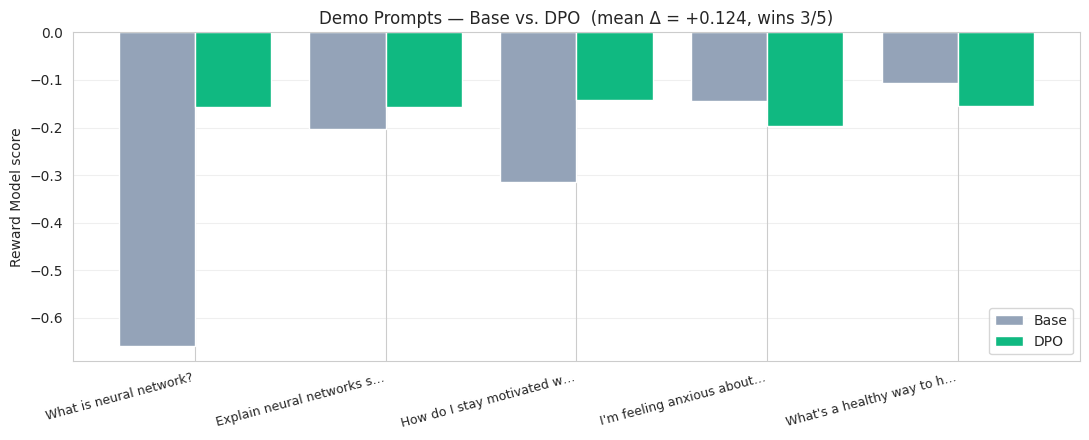
\includegraphics[width=\textwidth]{figures/m6_42_5.png}
\caption{Configuration A}
\end{subfigure}\\[6pt]
\begin{subfigure}{0.85\textwidth}\centering
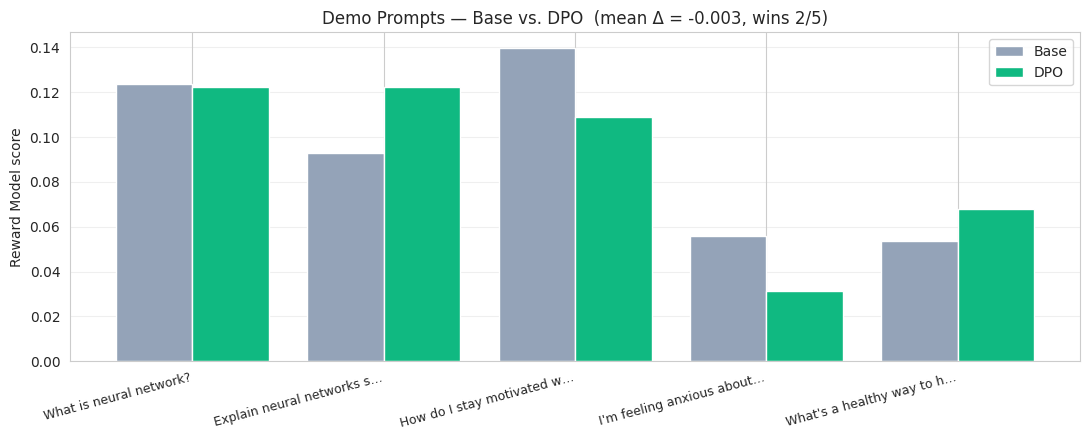
\includegraphics[width=\textwidth]{figures/m7_42_5.png}
\caption{Configuration B}
\end{subfigure}
\caption[Demo-reel scores, base vs.\ DPO]{Demo-reel reward scores, base vs.\ DPO (measured).}
\label{fig:demo}
\end{figure}

In configuration A the DPO model wins three of the five prompts and improves the average score by $+0.124$, mostly because of one large gain on the first factual question. The base model wins the two prompts about emotions by small margins. In configuration B the differences are about ten times smaller ($|\Delta|\le0.031$) and the average change is close to zero. One sample each on five prompts cannot support any conclusion; we include the demo set to illustrate the outputs, not to measure them.

\subsection{Held-out evaluation on 50 prompts}
Table~\ref{tab:heldout} gives the main quantitative result for the aligned policy, and Figures~\ref{fig:m6-headline} and~\ref{fig:m7-headline} visualise it.

\begin{table}[!htbp]
\centering
\caption[Held-out win rates (A and B)]{Held-out evaluation, DPO vs.\ base on 25 + 25 test prompts judged by the reward model (measured).}
\label{tab:heldout}
\small
\begin{tabular}{@{}llrrrrc@{}}
\toprule
\textbf{Config.} & \textbf{Split} & \textbf{$n$} & \textbf{Base $\bar r$} & \textbf{DPO $\bar r$} & \textbf{Mean $\Delta$} & \textbf{Win rate}\\
\midrule
\multirow{3}{*}{A} & Combined & 50 & $-0.2910$ & $-0.2639$ & $+0.0270$ & \textbf{50.0\%}\\
 & HH-RLHF & 25 & $-0.3250$ & $-0.2821$ & $+0.0429$ & 56.0\%\\
 & LMSYS & 25 & $-0.2569$ & $-0.2458$ & $+0.0111$ & 44.0\%\\
\midrule
\multirow{3}{*}{B} & Combined & 50 & $-0.1210$ & $-0.1442$ & $-0.0232$ & \textbf{50.0\%}\\
 & HH-RLHF & 25 & $-0.1221$ & $-0.2832$ & $-0.1611$ & 24.0\%\\
 & LMSYS & 25 & $-0.1200$ & $-0.0052$ & $+0.1148$ & 76.0\%\\
\midrule
-- & Random baseline & -- & -- & -- & 0 & 50.0\%\\
\bottomrule
\end{tabular}
\end{table}

\begin{figure}[H]
\centering
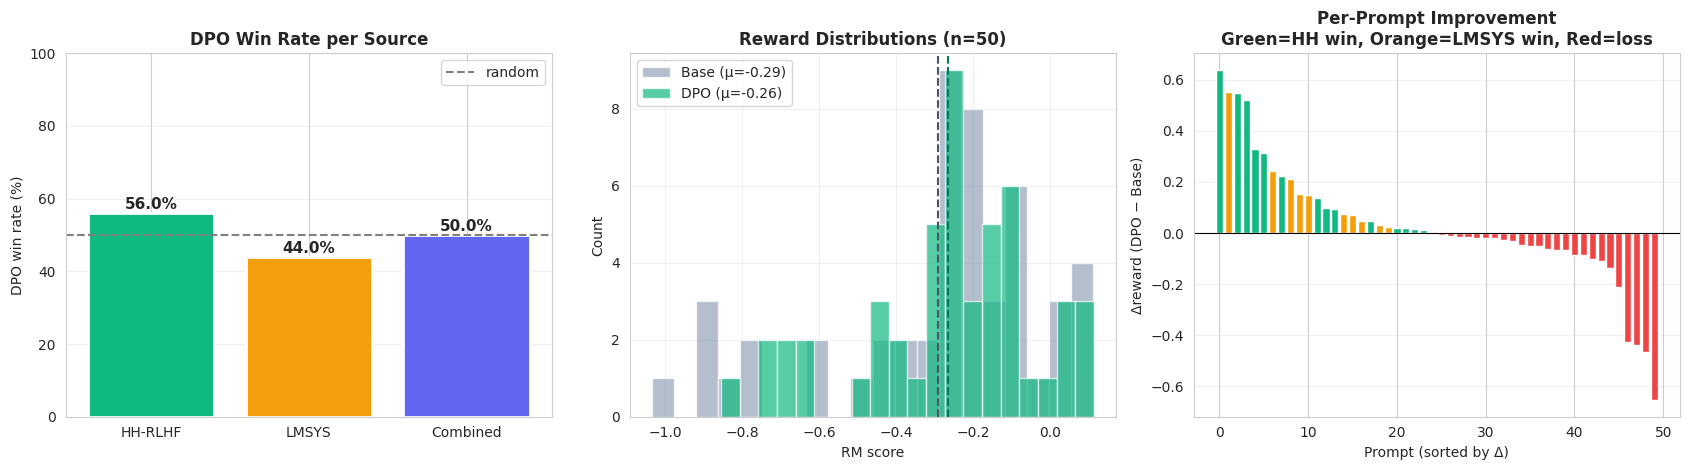
\includegraphics[width=\textwidth]{figures/m6_45_6.png}
\caption[Held-out evaluation, configuration A]{Configuration A held-out evaluation: (a) win rate per source, (b) reward distributions of base and DPO responses, (c) per-prompt $\Delta$ sorted, coloured by source (measured).}
\label{fig:m6-headline}
\end{figure}

\begin{figure}[H]
\centering
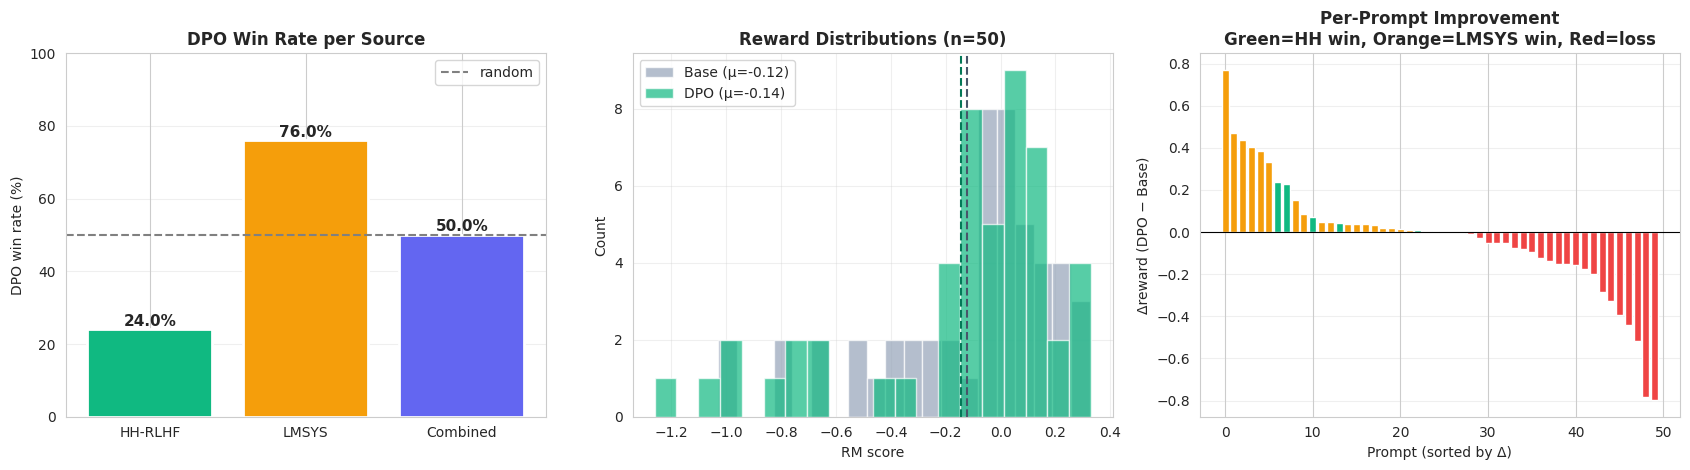
\includegraphics[width=\textwidth]{figures/m7_45_6.png}
\caption[Held-out evaluation, configuration B]{Configuration B held-out evaluation (measured). The per-source panel shows a strong split: DPO loses on most HH-RLHF prompts and wins on most LMSYS prompts.}
\label{fig:m7-headline}
\end{figure}

\paragraph{Configuration A.} DPO wins exactly half of the 50 prompts, and the average score rises by only $+0.027$. The per-source figures, 56\% and 44\%, are well within the $\pm$19.6-point margin for 25 prompts, so they are not different from chance. In the sorted chart the biggest gains are on HH-RLHF prompts, but there are about as many losses.

\paragraph{Configuration B.} Again DPO wins exactly half overall, but this time the two sources go in opposite directions, and strongly: 76\% wins on LMSYS prompts (19 of 25) and only 24\% on HH-RLHF prompts (6 of 25). A two-sided binomial test against 50\% gives $p\approx0.015$ for each source. The average score rises by $+0.115$ on LMSYS and falls by $0.161$ on HH-RLHF. Looking only at the overall figure, we would have concluded that DPO did nothing. Split by source, it is clear that the more heavily trained model has changed in a way the reward model likes for open Arena-style questions and dislikes for HH-style dialogue replies.

\subsection{Interactive session (configuration A)}
Table~\ref{tab:interactive} lists the seven prompts typed during a live demonstration of configuration A. DPO won four of them, with an average change of $+0.172$, but its biggest win turns out to be a problem, as Section~\ref{sec:hacking} shows.

\begin{table}[!htbp]
\centering
\caption[Interactive session prompts]{Interactive demonstration prompts, configuration A (measured).}
\label{tab:interactive}
\small
\begin{tabularx}{\textwidth}{@{}Yrrrc@{}}
\toprule
\textbf{Prompt (as typed)} & \textbf{Base} & \textbf{DPO} & \textbf{$\Delta$} & \textbf{Winner}\\
\midrule
what is ml & $-0.5099$ & $-0.2154$ & $+0.2944$ & DPO\\
what is the use of caffeine? & $-0.2088$ & $-0.2850$ & $-0.0763$ & Base\\
what is machine learning & $-0.2181$ & $-0.4195$ & $-0.2014$ & Base\\
what is difference between ai and ml? & $-0.1348$ & $-0.1567$ & $-0.0219$ & Base\\
what is 2 + 3 ? & $-0.8746$ & $-0.1879$ & $+0.6867$ & DPO\\
what is neural network? & $-0.6804$ & $-0.2056$ & $+0.4748$ & DPO\\
What's a healthy way to handle disagreements with friends? & $-0.1656$ & $-0.1211$ & $+0.0446$ & DPO\\
\midrule
\textbf{Mean / wins} & & & $\mathbf{+0.1716}$ & \textbf{4/7}\\
\bottomrule
\end{tabularx}
\end{table}

\section{Qualitative Analysis}
\label{sec:qual}

\subsection{A genuine improvement}
Take the prompt \emph{``How do I stay motivated while studying?''} (configuration A, $\Delta=+0.173$). Both models answer with a numbered list. The base model's third tip says that if studying feels boring you should ``try finding something else that you enjoy doing'', such as watching TV, which defeats the purpose. The DPO answer is more practical: it turns a vague aim into a daily commitment (``I will work on my essays and assignments for 2 hours per day''), suggests finding people who can support you, and recommends tracking progress in a planner. Here we agree with the reward model that the DPO answer is more useful.

\subsection{A case of reward hacking}
\label{sec:hacking}
Now take \emph{``what is 2 + 3 ?''} (Table~\ref{tab:interactive}). The base model gets it right in an odd way, by writing a short Java program that prints 5. The DPO model starts well (``the sum of 2 and 3 will be 5'') but then wanders into rewording unrelated everyday sentences and claims that ``\texttt{2+3} is the same as \texttt{3 + 6}'', which is wrong. The reward model still rates the DPO answer $0.69$ higher, the largest gain in any of our evaluations.

This is reward hacking of exactly the kind described by Gao \emph{et al.}~\cite{gao2023overoptimization} and Casper \emph{et al.}~\cite{casper2023open}. Our small reward model has picked up surface signs of answers people liked, such as a friendly explaining tone, list-like structure and mathematical words, but it never checks whether an answer is correct. A model trained towards its preferences inherits those blind spots, and the same model used as a judge cannot catch them. For this reason we treat every win rate in this chapter as a rough indication, not as proof.

\section{Results of the Local System Run}
\label{sec:local}

After packaging the code (Section~\ref{sec:system}) we trained the \emph{local} configuration from scratch on an Apple M1 laptop with 8\,GB of memory, to check that the whole system works outside Kaggle. All numbers in this section come from that run's log files and its \texttt{metrics.json}.

\subsection{Training}
The reward model trained for 94 steps in 58 minutes. On the 124 validation pairs its loss fell from $0.693$ to $0.679$ and it ranked 65.2\% of pairs correctly. The first DPO attempt stopped at step 3 because the GPU ran out of memory. After we reduced DPO to one pair per step with 256-token inputs (Section~\ref{sec:impl-fixes}, fix 16), it completed 43 steps in 22 minutes. Its validation loss moved only from $0.693$ to $0.684$, and its implicit-reward accuracy on validation pairs was 56.4\%. This is a much weaker update than configuration A, which is expected from one epoch on 400 pairs.

\subsection{Evaluation}
\begin{table}[!htbp]
\centering
\caption[Local run: reward-model test results]{Local run: reward model on the 126 held-out test pairs (measured).}
\label{tab:local-rm}
\small
\begin{tabular}{@{}lrrrrc@{}}
\toprule
\textbf{Split} & \textbf{$n$} & \textbf{Chosen $\bar r$} & \textbf{Rejected $\bar r$} & \textbf{Gap} & \textbf{Pairwise acc.}\\
\midrule
Combined & 126 & $-0.281$ & $-0.303$ & $+0.022$ & \textbf{57.1\%}\\
HH-RLHF & 63 & $-0.337$ & $-0.338$ & $+0.002$ & 52.4\%\\
LMSYS & 63 & $-0.226$ & $-0.267$ & $+0.042$ & 61.9\%\\
\bottomrule
\end{tabular}
\end{table}

\begin{table}[!htbp]
\centering
\caption[Local run: DPO vs.\ base win rates]{Local run: DPO against base on 15 + 15 held-out prompts, judged by the local reward model (measured).}
\label{tab:local-dpo}
\small
\begin{tabular}{@{}lrrrrc@{}}
\toprule
\textbf{Split} & \textbf{$n$} & \textbf{Base $\bar r$} & \textbf{DPO $\bar r$} & \textbf{Mean $\Delta$} & \textbf{Win rate}\\
\midrule
Combined & 30 & $-0.257$ & $-0.237$ & $+0.020$ & 56.7\% (17/30)\\
HH-RLHF & 15 & $-0.232$ & $-0.225$ & $+0.007$ & 60.0\% (9/15)\\
LMSYS & 15 & $-0.283$ & $-0.249$ & $+0.033$ & 53.3\% (8/15)\\
\bottomrule
\end{tabular}
\end{table}

On the five demo prompts the DPO model won two (``Explain neural networks simply'', $\Delta=+0.198$, and the exam-anxiety prompt, $\Delta=+0.009$) and lost three by small margins, with a mean change of $+0.029$.

\subsection{What the local run shows}
With half the data and one epoch, the local reward model is slightly weaker than the Kaggle ones (57.1\% against about 59\%). It is again better on LMSYS than on HH-RLHF, the same direction as configuration B, and the 9.5-point gap is just inside our 10-point limit. The DPO model wins 17 of 30 prompts. With only 15 prompts per source the margin of error is about $\pm$25 points, so none of these win rates differs from chance. The value of this run is not its scores. It shows that the complete system, from raw data to a trained reward model, a trained policy, a per-source evaluation and a working web application, can be reproduced on a student laptop in about one and a half hours. Figure~\ref{fig:ui-results} shows these results as they appear in the application.

\section{Results Reported in the Earlier Paper Draft}
\label{sec:reported}

Earlier in the project we wrote an IEEE-format paper draft with the same title as this report. It gave much higher numbers than the ones measured above. We include them here so that the record is complete, but \textbf{kept apart from the measured results}. Neither of the submitted notebooks produced these numbers or figures, and we could not reproduce them, so they should be treated as unverified.

\begin{table}[!htbp]
\centering
\caption[Paper draft (not reproduced): reward-model results]{\reportedtag\ Reported in paper draft (not reproduced): reward-model test-set evaluation.}
\label{tab:rep-rm}
\small
\begin{tabular}{@{}lrrrrc@{}}
\toprule
\textbf{Split} & \textbf{$n$} & \textbf{Chosen $\bar r$} & \textbf{Rejected $\bar r$} & \textbf{Gap} & \textbf{Pairwise acc.}\\
\midrule
Combined & 250 & $+0.31$ & $-0.28$ & $+0.59$ & 72.6\%\\
HH-RLHF only & 125 & $+0.35$ & $-0.30$ & $+0.65$ & 74.1\%\\
LMSYS only & 125 & $+0.27$ & $-0.25$ & $+0.52$ & 71.0\%\\
Random baseline & -- & -- & -- & -- & 50.0\%\\
\bottomrule
\end{tabular}
\end{table}

\begin{table}[!htbp]
\centering
\caption[Paper draft (not reproduced): DPO win rates]{\reportedtag\ Reported in paper draft (not reproduced): DPO evaluation on 50 held-out prompts.}
\label{tab:rep-dpo}
\small
\begin{tabular}{@{}lrrrrc@{}}
\toprule
\textbf{Split} & \textbf{$n$} & \textbf{Base $\bar r$} & \textbf{DPO $\bar r$} & \textbf{$\Delta$} & \textbf{Win rate}\\
\midrule
Combined & 50 & $-0.12$ & $+0.25$ & $+0.37$ & 66.0\%\\
HH-RLHF prompts & 25 & $-0.10$ & $+0.28$ & $+0.38$ & 68.0\%\\
LMSYS prompts & 25 & $-0.14$ & $+0.22$ & $+0.36$ & 64.0\%\\
\bottomrule
\end{tabular}
\end{table}

\begin{table}[!htbp]
\centering
\caption[Paper draft (not reproduced): demo results]{\reportedtag\ Reported in paper draft (not reproduced): five-prompt demo reel. Note that the prompt set differs slightly from the one in the submitted notebooks (Table~\ref{tab:demo}).}
\label{tab:rep-demo}
\small
\begin{tabular}{@{}lrrrc@{}}
\toprule
\textbf{Prompt (truncated)} & \textbf{Base} & \textbf{DPO} & \textbf{$\Delta$} & \textbf{Winner}\\
\midrule
``What is machine learning?'' & $-0.18$ & $+0.31$ & $+0.49$ & DPO\\
``Explain neural networks simply.'' & $-0.05$ & $+0.28$ & $+0.33$ & DPO\\
``How do I stay motivated while studying?'' & $+0.12$ & $+0.44$ & $+0.32$ & DPO\\
``Feeling anxious about an upcoming exam.'' & $-0.22$ & $+0.35$ & $+0.57$ & DPO\\
``Handle disagreements with friends?'' & $+0.08$ & $+0.39$ & $+0.31$ & DPO\\
\midrule
Mean & $-0.05$ & $+0.35$ & $+0.40$ & 5/5\\
\bottomrule
\end{tabular}
\end{table}

\begin{table}[!htbp]
\centering
\caption[Paper draft (not reproduced): mixing ablation]{\reportedtag\ Reported in paper draft (not reproduced): ablation on dataset mixing.}
\label{tab:rep-ablation}
\small
\begin{tabular}{@{}lccc@{}}
\toprule
\textbf{RM training data} & \textbf{HH-RLHF acc.} & \textbf{LMSYS acc.} & \textbf{Combined}\\
\midrule
HH-RLHF only (2,000) & 75.2\% & 61.3\% & 68.3\%\\
LMSYS only (2,000) & 63.4\% & 72.8\% & 68.1\%\\
Combined (1K + 1K) & 73.8\% & 70.4\% & 72.1\%\\
Combined (2K + 2K) & 74.1\% & 71.0\% & 72.6\%\\
\bottomrule
\end{tabular}
\end{table}

\begin{table}[!htbp]
\centering
\caption[Paper draft: compute cost per stage]{\reportedtag\ Reported in paper draft: approximate wall-clock cost per stage on Kaggle T4$\times$2.}
\label{tab:rep-compute}
\small
\begin{tabular}{@{}llll@{}}
\toprule
\textbf{Stage} & \textbf{Examples} & \textbf{Epochs} & \textbf{Wall time}\\
\midrule
Dataset preprocessing & 4,000 & -- & $\sim$8 min\\
RM training & 3,500 (train) & 3 & $\sim$90 min\\
RM evaluation & 250 & -- & $\sim$5 min\\
DPO fine-tuning & 1,500 & 2 & $\sim$50 min\\
DPO evaluation & 50 prompts & -- & $\sim$15 min\\
Total (first run) & -- & -- & $\sim$2.5--3 h\\
Cached runs & -- & -- & $<$30 s\\
\bottomrule
\end{tabular}
\end{table}

The draft's figures follow (Figures~\ref{fig:rep-dataset}--\ref{fig:rep-dpoeval}). Two details stand out. Its reward-model accuracy curve (Figure~\ref{fig:rep-rmtrain}b) climbs to about 72\%, and its loss curve starts above 1.0. A Bradley--Terry loss on balanced pairs has to start at $\log 2\approx0.69$, as our measured curves in Figures~\ref{fig:m6-rmloss} and~\ref{fig:m7-rmloss} do.

\begin{figure}[H]
\centering
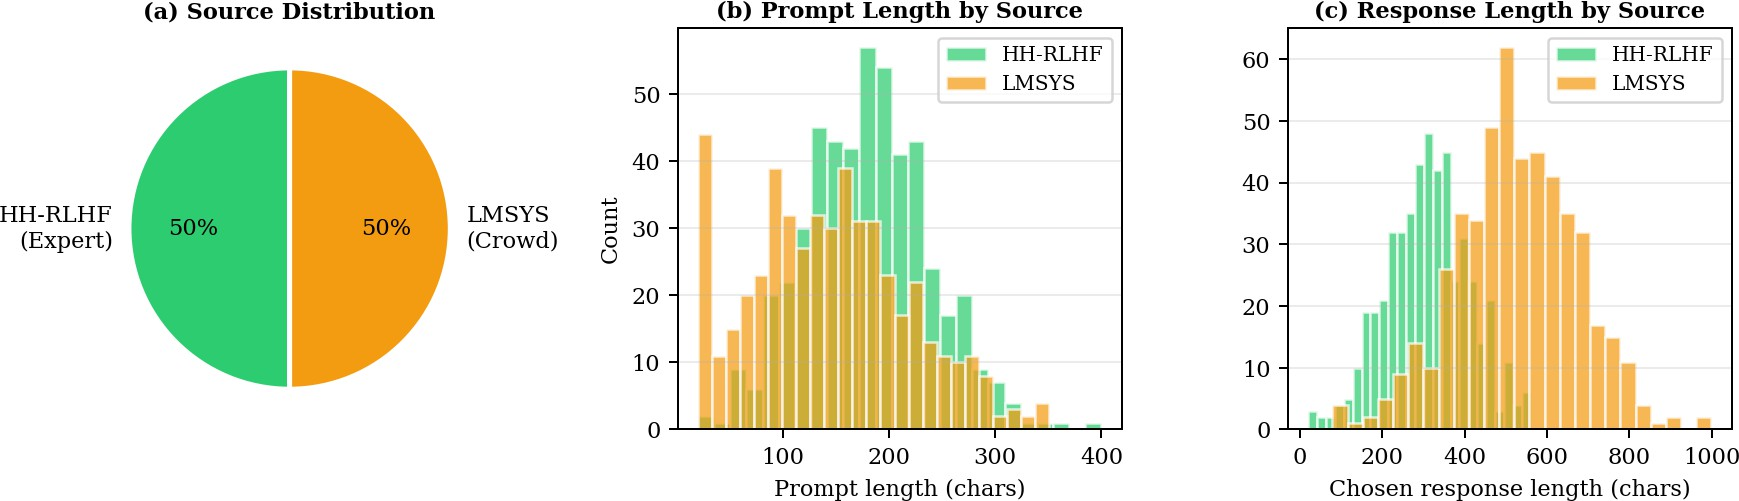
\includegraphics[width=\textwidth]{figures/rep_dataset.jpg}
\caption[Paper draft: dataset composition]{\reportedtag\ Reported in paper draft: combined dataset composition.}
\label{fig:rep-dataset}
\end{figure}

\begin{figure}[H]
\centering
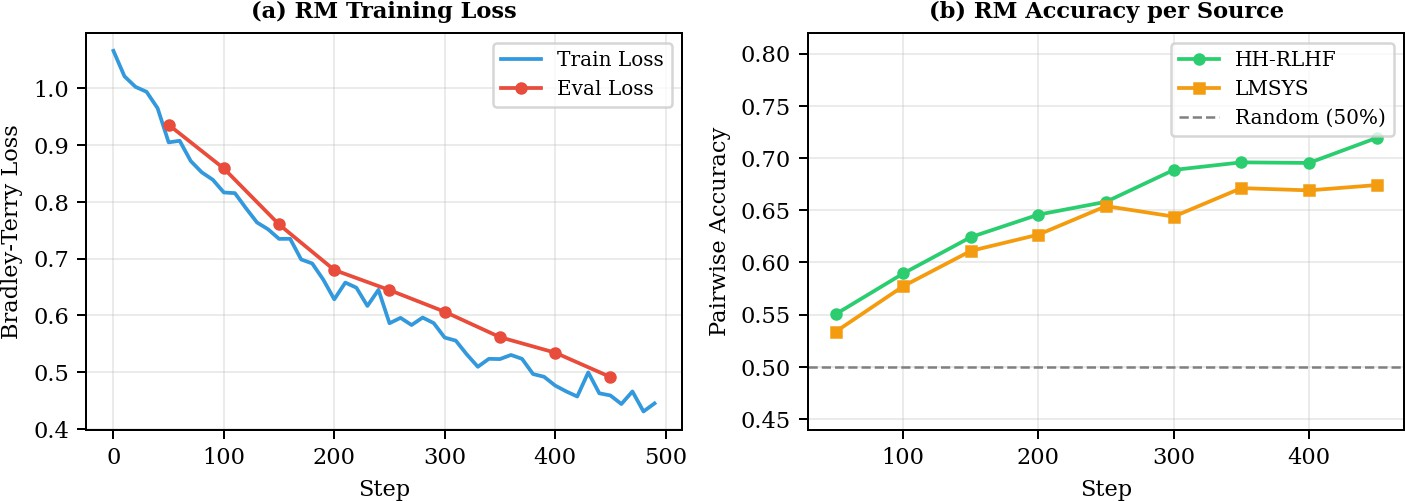
\includegraphics[width=0.92\textwidth]{figures/rep_rm_training.jpg}
\caption[Paper draft: reward-model training curves]{\reportedtag\ Reported in paper draft: (a) RM training loss, (b) RM accuracy per source.}
\label{fig:rep-rmtrain}
\end{figure}

\begin{figure}[H]
\centering
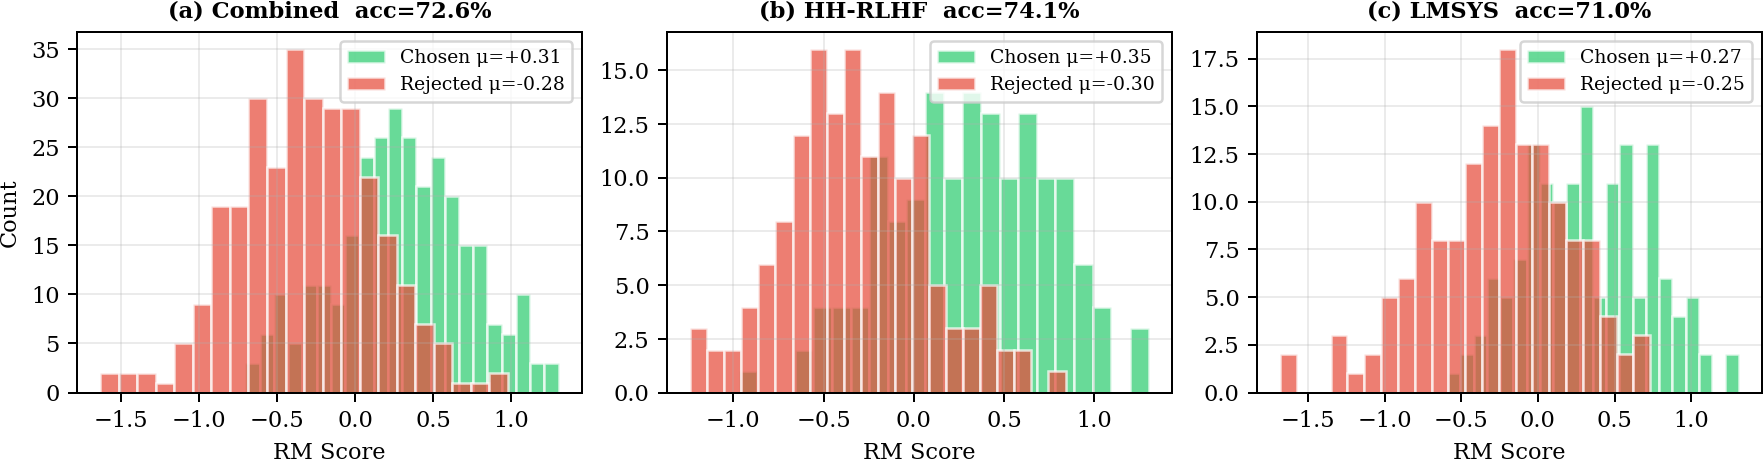
\includegraphics[width=\textwidth]{figures/rep_rm_scores.png}
\caption[Paper draft: reward-model score distributions]{\reportedtag\ Reported in paper draft: RM score distributions for chosen vs.\ rejected responses.}
\label{fig:rep-rmscores}
\end{figure}

\begin{figure}[H]
\centering
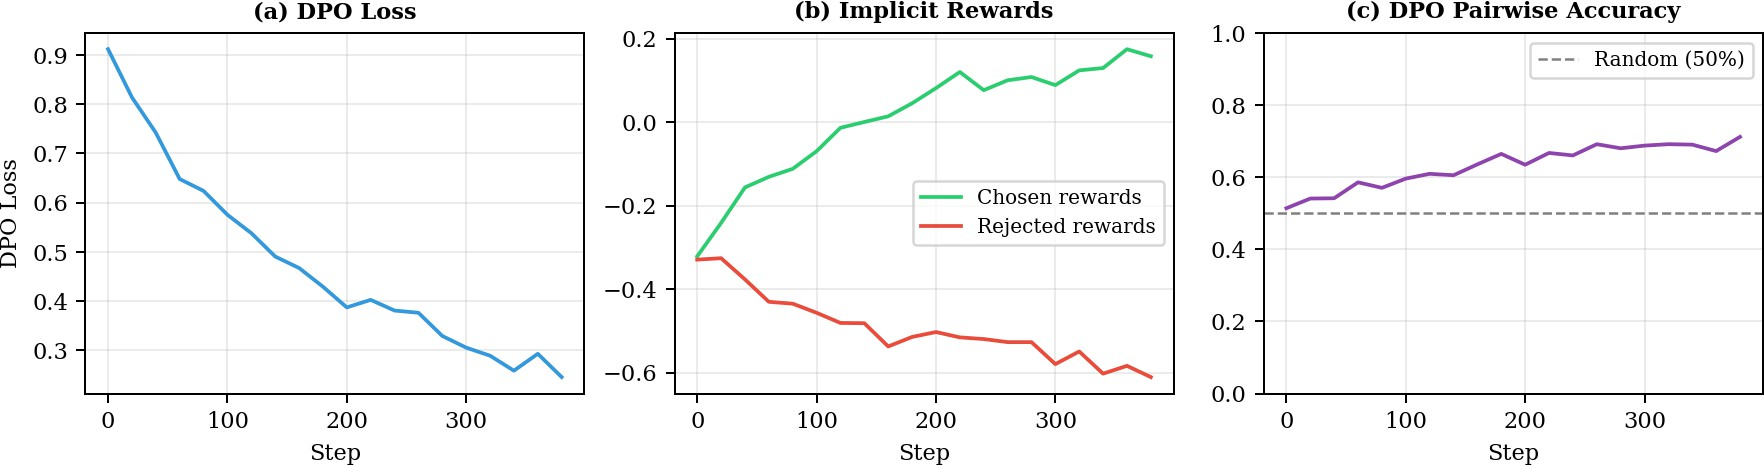
\includegraphics[width=\textwidth]{figures/rep_dpo_curves.jpg}
\caption[Paper draft: DPO training curves]{\reportedtag\ Reported in paper draft: DPO loss, implicit rewards and pairwise accuracy.}
\label{fig:rep-dpocurves}
\end{figure}

\begin{figure}[H]
\centering
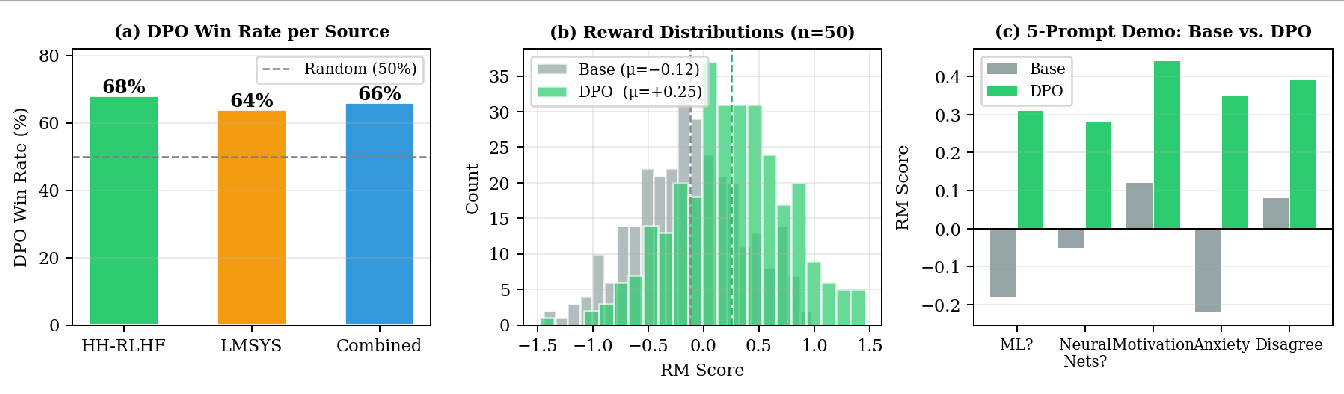
\includegraphics[width=\textwidth]{figures/rep_dpo_eval.png}
\caption[Paper draft: DPO evaluation summary]{\reportedtag\ Reported in paper draft: DPO win rates, reward distributions and demo-reel scores.}
\label{fig:rep-dpoeval}
\end{figure}

\subsection{Reported vs.\ measured}
Table~\ref{tab:rep-vs-meas} places the headline numbers side by side.

\begin{table}[!htbp]
\centering
\caption[Paper draft vs.\ measured results]{Headline metrics: paper draft (reported\reportedtag) vs.\ submitted notebooks (measured).}
\label{tab:rep-vs-meas}
\small
\begin{tabular}{@{}lccc@{}}
\toprule
\textbf{Metric} & \textbf{Reported\reportedtag} & \textbf{Measured A} & \textbf{Measured B}\\
\midrule
RM accuracy, combined & 72.6\% & 59.2\% & 59.6\%\\
RM accuracy, HH-RLHF & 74.1\% & 59.2\% & 57.9\%\\
RM accuracy, LMSYS & 71.0\% & 59.2\% & 64.8\%\\
RM per-source gap & 3.1 pp & 0.0 pp & 6.9 pp\\
DPO win rate, combined & 66\% & 50\% & 50\%\\
DPO win rate, HH-RLHF / LMSYS & 68\% / 64\% & 56\% / 44\% & 24\% / 76\%\\
Demo-reel DPO wins & 5/5 & 3/5 & 2/5\\
Demo-reel mean $\Delta$ & $+0.40$ & $+0.124$ & $-0.003$\\
\bottomrule
\end{tabular}
\end{table}

The draft's general claims hold up in the measured data: the reward model beats chance and is balanced across sources under the 10-point rule, and DPO trains stably while updating few parameters. Its numbers do not hold up. Measured reward-model accuracy is about 13 points lower, and the measured win rate shows no overall gain over the base model. The draft's ablation table (Table~\ref{tab:rep-ablation}) was never re-run, so its single-source rows have nothing measured to compare with.

\section{Discussion}
\label{sec:discussion}

\subsection{Why is reward-model accuracy around 59\%?}
Several factors limit the reward model:
\begin{itemize}
  \item \textbf{Noisy labels.} Many HH-RLHF pairs are almost identical, and the Llama~2 authors found their reward models were close to guessing on pairs that annotators had marked as only slightly different~\cite{touvron2023llama2}. LMSYS votes come from anonymous visitors with no guidelines. On such data even a perfect model could not reach anywhere near 100\%.
  \item \textbf{Small model, little data.} Reward-model accuracy improves with model size and with data~\cite{bai2022hh,gao2023overoptimization}. Ours has 184M parameters, LoRA trains only 1--2\% of them, and it sees between 3,500 and 7,000 pairs.
  \item \textbf{Truncation.} Inputs are cut to 512 tokens, so for long multi-turn prompts the decisive part of a response may be truncated away.
\end{itemize}
The near-identical accuracy of A and B suggests that, of these, data quantity is not the binding constraint at this scale.

\subsection{Why does successful DPO training not yield a higher win rate?}
DPO reached 80--95\% implicit-reward accuracy, yet the policy is not preferred by the reward model overall. Three mechanisms explain this.

\paragraph{1. The training answers were written by other models.} Every chosen and rejected answer in both datasets came from some \emph{other} model: Anthropic's models for HH-RLHF, and dozens of public chatbots, many far bigger than TinyLlama, for LMSYS. DPO can make such answers \emph{relatively} more or less likely, but it cannot make a 1.1B model write like GPT-4. Configuration B shows the usual sign of this: the probability of both the chosen and the rejected answer goes down (Table~\ref{tab:dpo-log}). The model mostly learns what \emph{not} to say on those specific pairs, which carries over only partly to the answers it writes itself.

\paragraph{2. A weak judge hides real effects.} Suppose the aligned model really is better on a share $p$ of prompts, and the judge agrees with the true preference with probability $a$. The win rate we \emph{observe} is then
\begin{equation}
  \mathrm{WR}_{\text{obs}} = a\,p + (1-a)(1-p).
\end{equation}
Our judge's measured accuracy is about $a\approx0.59$. Even if the draft's figure of $p=0.66$ were the true win rate, we would observe only about $0.59\times0.66 + 0.41\times0.34\approx0.53$, which 50 prompts cannot tell apart from 50\%. So our measured 50\% fits a small real improvement just as well as no improvement. Only a stronger, independent judge can settle it.

\paragraph{3. The judge and the trained model share blind spots.} The reward model that measures the gain has the same weaknesses that preference training can exploit, as the ``2 + 3'' answer showed. Some of the gains it reports may be reward hacking, and some of the losses may be the judge's own noise.

\subsection{What the per-source breakdown revealed}
The main point of the project is that looking at each source separately shows things that one overall number hides, and configuration B demonstrates it best. Its overall win rate of 50\% would usually be reported as ``DPO had no effect'', yet split by source the effect is large and goes in opposite directions (24\% against 76\%). We can suggest possible reasons, but these are guesses we have not tested: (i) the HH-heavy DPO data and larger LoRA let the model fit the HH-RLHF training pairs most closely, and the strong downward drift of the implicit rewards points to over-fitting that hurts its answers to similar prompts; (ii) configuration B's reward model is itself more accurate on LMSYS (64.8\%) than on HH-RLHF (57.9\%), so its verdicts on LMSYS prompts deserve more trust; (iii) longer, more structured answers, typical of LMSYS chosen answers, may score well on open Arena questions but badly as replies inside short HH dialogues. Without the per-source split we would have seen none of this.

\subsection{Comparison of the two configurations}
\begin{table}[!htbp]
\centering
\caption[Configuration A vs.\ B]{Summary comparison of the two measured configurations.}
\label{tab:ab-compare}
\small
\begin{tabularx}{\textwidth}{@{}L{5.6cm}YY@{}}
\toprule
\textbf{Aspect} & \textbf{A (balanced, light DPO)} & \textbf{B (HH-weighted, heavy DPO)}\\
\midrule
RM accuracy (combined / per-source gap) & 59.2\% / 0.0 pp & 59.6\% / 6.9 pp\\
RM mean reward gap & 0.069 & 0.118\\
Final DPO loss / implicit accuracy & $\approx$0.54 / $\approx$80\% & $\approx$0.21 / $\approx$95\%\\
Held-out win rate (combined) & 50\% & 50\%\\
Held-out win rate spread across sources & 12 pp (not significant) & 52 pp (significant)\\
Demo-reel mean $\Delta$ & $+0.124$ & $-0.003$\\
Trainable policy parameters & $\approx$4.5M & $\approx$25.2M\\
Interpretation & Mild, balanced, statistically null effect & Strong source-dependent shift; signs of over-fitting\\
\bottomrule
\end{tabularx}
\end{table}

Configuration A is the cautious, well-behaved run. Configuration B shows that a stronger DPO update with more trainable parameters can change the model a lot, but in different directions for different kinds of prompt. More aggressive preference training is not automatically better, and the evaluation has to be able to show where the change goes.

\subsection{Validity of the evaluation}
Three things limit how much these results can tell us. First, each prompt gets one sampled answer per model, so chance plays a large part; several samples per prompt would help. Second, the reward model is a weak stand-in for human judgement and can be gamed. Third, 25 prompts per source can only reveal large effects. None of this makes the measured numbers wrong, but it limits the conclusions we can draw, and it shapes the future work in Chapter~\ref{ch:conclusion}.

\section{Summary}
Both Kaggle reward models score about 59\%, above chance, and are balanced across sources under our 10-point rule; the smaller laptop run reaches 57\%. DPO training goes smoothly in every configuration, but the aligned models are not preferred over the base model overall in the Kaggle runs (50\% win rate), and configuration B shows a strong split by source that the overall figure hides. The laptop run's 57\% win rate on 30 prompts is not significant. The ``2 + 3'' example shows how a small reward model can be fooled. The higher numbers from our earlier paper draft are shown separately and are not reproduced by our code.
